\documentclass[11pt]{article}

\usepackage[left=1.25in,top=1.25in,right=1.25in,bottom=1.25in,head=1.25in]{geometry}
\usepackage{amsfonts,amsmath,amssymb,amsthm}
\usepackage{cite}
\usepackage[shortlabels]{enumitem}
\usepackage{xcolor}
\usepackage[ruled,vlined,linesnumbered]{algorithm2e}
\usepackage{url}
\usepackage[colorlinks=true,linkcolor=blue]{hyperref}
\newsavebox{\mycode}
\usepackage{graphicx}
\usepackage{setspace}
\usepackage{caption}


\title{Summary and discussion of: "Flexible Signal Denoising via Flexible Empirical Bayes Shrinkage" }
% \large Journal club report}
\author{RUIZHAO HUANG}
\date{}

\begin{document}
\maketitle

\section{Summary}
	
\subsection{Empirical Bayes for Normal Mean}
This section corresponds to the concepts covered in the lecture. Let us assume we have a set of observations, denoted as $\boldsymbol{z} = (z_1, \ldots, z_N)^T$, where:
$$
z_i \vert \mu_i \stackrel{\text{i.i.d.}}{\sim} \mathcal{N}(\mu_i, 1), \ \  i = 1, \ldots, N 
$$

In a compact matrix form, we have:
$$
\boldsymbol{z} \vert \boldsymbol{\mu} \stackrel{\text{}}{\sim} \mathcal{N}(\boldsymbol{\mu}, \mathbf{I}_N)
$$


Here, $\boldsymbol{\mu} = (\mu_1, \ldots, \mu_N)^T$ are unknown, and want to estimate. If we assume homoskedastic Gaussian prior to $\boldsymbol{\mu}$, such that:
$$
\mu_i \stackrel{\text{i.i.d.}}{\sim} \mathcal{N}(0, \sigma^2), \ \ i = 1, \ldots, N 
$$

In a compact matrix form, we have:
$$
\boldsymbol{\mu} \stackrel{\text{}}{\sim} \mathcal{N}(\boldsymbol{\mu}, \sigma^2 \mathbf{I}_N)
$$


Under these assumptions, the marginal distribution of $\boldsymbol{z}$ will be:
$$
\boldsymbol{z}  \stackrel{\text{}}{\sim} \mathcal{N} \bigl(\boldsymbol{\mu}, (1 + \sigma^2) \mathbf{I}_N \bigl) 
$$

The general Empirical Bayes method to estimate $\boldsymbol{\mu}$ in this case can be summarized in the following two steps:
\begin{enumerate}[a)]
\item Get the estimate of $\sigma^2$ by maximize the marginal likelihood of $\boldsymbol{z}$, which is adaptively estimated from data.
\item Incorporate the estimated value of $\sigma^2$ and derive the posterior distribution of $\boldsymbol{\mu}$. The estimation of $\boldsymbol{\mu}$ can be obtained using either the posterior mean or median.
\end{enumerate}

It is worth to note that in this case, we can leverage the distributional information of $\boldsymbol{z}$ and its relationship with $(1 + \sigma^2)$, such that $\sum_{i=1}^N \frac{z_i^2}{1+\sigma^2} \sim \chi_N^2$. Consequently, the order of the above procedure is actually reversed. However, for consistency with subsequent cases, I have presented it in this order.


\subsection{Empirical Bayes for Sparse Normal Mean}
Next, within the framework established in the previous section, we consider the scenario where $\boldsymbol{\mu}$ is assumed to be sparse. To tackle this case, I will outline the method proposed by the author in another paper called \verb|ASH| \cite{Stephens} --- this method serves as a fundamental component of the approach introduced in this paper, which is called \verb|SMASH| \cite{Xing}. 

The major differences of \verb|ASH| with previous section are as following:
\begin{enumerate}[a)]
\item Instead of assuming a homoskedastic Gaussian prior, we consider the individual components of $\boldsymbol{\mu}$ to have a unimodal (mixture) prior, such that:
\begin{equation}
\mu_i \stackrel{\text{indep}}{\sim} \pi_0 \delta_0(\mu_i) + \sum_{i=1}^K \pi_k \mathcal{N}(\mu_i; 0, \sigma_k^2), \quad i = 1, \ldots, N, \quad \sum_{k=0}^K \pi_k = 1 
\label{ASH_assumption1}
\end{equation}
where $\delta_0$ represents the point mass at 0. This prior choice intuitively captures our knowledge regarding the sparsity of $\boldsymbol{\mu}$, allowing for the possibility that some $\mu_i$ values are exactly 0 with a certain probability $\pi_0$.

\item Instead of assuming $z_i \vert \mu_i \stackrel{\text{i.i.d.}}{\sim} \mathcal{N}(\mu_i, 1)$, we consider the following assumption:
\begin{equation}
z_i \vert \mu_i \stackrel{\text{indep}}{\sim} \mathcal{N}(z_i; \mu_i, \hat{s}_i^2) \quad \Longrightarrow \quad \boldsymbol{z} \vert \boldsymbol{\mu} \stackrel{\text{}}{\sim} \mathcal{N}(\boldsymbol{z}; \boldsymbol{\mu}, \hat{\boldsymbol{S}}), \ \hat{\boldsymbol{S}} = \text{diag}(\hat{s}_1^2, \ldots, \hat{s}_N^2) 
\label{ASH_assumption2}
\end{equation}
where $\hat{s_i}^2$ represents the estimated variance of $z_i \vert \mu_i$, and its value is provided.
\item The parameters $\boldsymbol{\sigma} = (\sigma_1, \ldots, \sigma_K)$ are estimated using a grid search approach during the maximization of the marginal log-likelihood of $\boldsymbol{z}$. The grid resolution is set to be:
$$
\sigma_{min} = \frac{\min\{\hat{s}_i\}}{10}, \quad \sigma_{max} =  2 \sqrt{\max \left\{ \hat{z}_i^2-\hat{s}_i^2\right \} }, \quad \sigma_k= \sqrt{2} \sigma_{k-1}
$$ 
\end{enumerate}


Under these assumptions, the marginal density of $z_i$ are mixture Normal, and can be expressed as:
$$
p(z_i)  = \sum_{k=0}^K \pi_k \mathcal{N} \bigl(z_i; 0, \hat{s}_i^2+\sigma_k^2 \bigl), \ \ \sigma_0^2 = 0, \ \ i = 1, \ldots, N
$$

The marginal log-likelihood of $\boldsymbol{z}$ can be defined as:
$$
l(\boldsymbol{z}) =  \sum_{i=1}^N  \ln \Biggl( \sum_{k=0}^K \pi_k \mathcal{N} \bigl(z_i; 0, \hat{s}_i^2+\sigma_k^2 \bigl) \Biggl)
$$


It is worth noting that since we employ a grid search to estimate $\sigma_k^2$, which treats $\sigma_k^2$ as fixed, the function $L(\boldsymbol{z}, \boldsymbol{\pi})$ is concave with respect to $\boldsymbol{\pi}$. This is a result of the concavity of the logarithm function and the fact that a non-negative weighted concave function remains concave.

Thus, the optimal solution for $\boldsymbol{\pi}$ can be obtained by solving the following convex optimization problem:
$$
\begin{array}{ll}
\underset{\boldsymbol{\pi}}{\operatorname{Maximize}} &  \sum_{i=1}^N  \ln \Bigl( \sum_{k=0}^K \pi_k \mathcal{N} \bigl(z_i; 0, \hat{s}_i^2+\sigma_k^2 \bigl) \Bigl)  \\
\text { subject to } &  \mathbf{1}^T \boldsymbol{\pi} = 1, \ \  \boldsymbol{\pi} \succeq \mathbf{0}
\end{array}
$$

However, this paper considers the following penalized convex optimization problem:
$$
\begin{array}{ll}
\underset{\boldsymbol{\pi}}{\operatorname{Maximize}} &  \sum_{i=1}^N  \ln \Bigl( \sum_{k=0}^K \pi_k \mathcal{N} \bigl(z_i; 0, \hat{s}_i^2+\sigma_k^2 \bigl) \Bigl) + \sum_{k=0}^K\left(\lambda_k-1\right) \ln \pi_k \\
\text { subject to } &  \mathbf{1}^T \boldsymbol{\pi} = 1, \ \  \boldsymbol{\pi} \succeq \mathbf{0}
\end{array}
$$

The default settings are $\lambda_0 = 10$, and $\lambda_k = 1$ for $k > 0$. It is important to note that under this setting, $\lambda_k - 1 = 0$ for $k>0$, and since we are maximizing the objective function, the optimization process will tend to push $\pi_0$ away from 0, which can be interpreted as an over-estimation of $\pi_0$ to encourage sparsity.

Alternatively, we can use the EM algorithm to estimate $\boldsymbol{\pi}$, as the marginal density of $z_i$ follow the mixture Normal distribution. To do this, let's introduce a latent variable $\boldsymbol{x}_i = (x_{i0}, \ldots, x_{iK})$ defined as:
$$
\mathbb{P}(x_{ik} = 1) = \pi_k, \ \ 0 \leqslant \pi_k \leqslant 1, \ \ \sum_{k=0}^K \pi_k = 1
$$

Consequently, we can express the joint distribution of $\boldsymbol{x}$ and $z_i$ compactly as follows:
$$
p(\boldsymbol{x}_i, z_i) = \prod_{k=0}^K \Bigl( \pi_k \mathcal{N} \bigl(z_i; 0, \hat{s}_i^2+\sigma_k^2 \bigl) \Bigl)^{x_{ik}}, \quad i = 1, \ldots, N
$$

% Then, the complete likelihood of $(\boldsymbol{x}, \boldsymbol{z})$ is:
% $$
% p(\boldsymbol{x}, \boldsymbol{z}) = \prod_{i=1}^N \prod_{k=1}^K \Bigl( \pi_k \mathcal{N} \bigl(0, \hat{s_i}^2+\sigma_k^2 \bigl) \Bigl)^{x_{k}}
% $$

Next, the complete log-likelihood of $(\boldsymbol{x}, \boldsymbol{z})$ is given by:
$$
\ln p(\boldsymbol{x}, \boldsymbol{z}) = \sum_{i=1}^N \sum_{k=0}^K x_{ik} \Bigl( \ln{\pi_k} + \ln \mathcal{N} \bigl(z_i; 0, \hat{s}_i^2+\sigma_k^2 \bigl) \Bigl)
$$

Suppose we have the previous parameter $\boldsymbol{\pi}^{\text{old}}$, then the expectation of the complete log-likelihood with respect to the posterior distribution of the latent variable $\boldsymbol{x}$ at $\boldsymbol{\pi}^{\text{old}}$ is:
$$
\begin{aligned}
& \mathbb{E}_{\boldsymbol{x} \vert \mathbf{z}, \boldsymbol{\pi}^{\text{old}}} \Bigl( \ln p(\boldsymbol{x}, \boldsymbol{z}) \Big) = \sum_{i=1}^N \sum_{k=1}^K \mathbb{E}_{\boldsymbol{x} \vert \mathbf{z}, \boldsymbol{\pi}^{\text{old}}}(x_{ik}) \Bigl( \ln{\pi_k} + \ln \mathcal{N} \bigl(z_i; 0, \hat{s}_i^2+\sigma_k^2 \bigl) \Bigl)
\end{aligned}
$$


Since $x_{ik}$ is a Bernoulli random variable, we have:
$$
\begin{aligned}
\gamma(x_{ik}) & : = \mathbb{E}_{\boldsymbol{x} \vert \mathbf{z}, \boldsymbol{\pi}^{\text{old}}}(x_{ik}) = \mathbb{P}_{\boldsymbol{x}} \bigl(x_{ik} = 1 \vert z_i, \boldsymbol{\pi}^{\text{old}} \bigl)  \\ 
& = \frac{\pi_k \mathcal{N} \bigl(z_i; 0, \hat{s}_i^2+\sigma_k^2 \bigl)}{\sum_{j=0}^K \pi_j \mathcal{N} \bigl(z_i; 0, \hat{s}_i^2+\sigma_j^2 \bigl)}
\end{aligned}
$$


Furthermore, in the maximization step, we need to incorporate the penalty term, resulting in the following convex optimization problem:
$$
\begin{array}{ll}
\underset{\boldsymbol{\pi}}{\operatorname{Maximize}} &  \sum_{i=1}^N \sum_{k=0}^K \gamma(x_{ik}) \Bigl(  \ln{\pi_k} + \ln \mathcal{N} \bigl(z_i; 0, \hat{s}_i^2+\sigma_k^2 \bigl) \Bigl) + \sum_{k=0}^K\left(\lambda_k-1\right) \ln \pi_k \\
\text { subject to } &  \mathbf{1}^T \boldsymbol{\pi} = 1, \ \  \boldsymbol{\pi} \succeq \mathbf{0}
\end{array}
$$


To solve this convex optimization problem, note that we can optimize each coordinate individually (for each $k$) since they are separable. We can utilize Lagrangian multipliers of $\pi_k \geqslant 0$ along with the equality constraint $\mathbf{1}^T \boldsymbol{\pi} = 1$ to solve the problem. The optimal solution is given by:
$$
\pi_k^{*} = \frac{\sum_{i=1}^N\gamma(x_{ik}) + \lambda_k - 1}{\sum_{k=0}^K \Bigl( \sum_{i=1}^N\gamma(x_{ik}) + \lambda_k - 1 \Bigl)}
$$


\begin{algorithm}[H]
\begin{lrbox}{\mycode}
\verb!ASH!
\end{lrbox}
\SetAlgoLined
\KwData{Given $\boldsymbol{z}$, $\boldsymbol{\sigma}^2$, $\sigma_0^2 = 0$, $\hat{\boldsymbol{s}}^2$;}
% \KwResult{how to write algorithm with \LaTeX2e}
Initialization: $\pi_k = 1/N$ for $k = 1, \ldots, K$, $\pi_0 = 1 - \sum_{k=1}^K \pi_k$ \;
Evaluate the incomplete log-likelihood $\ln p ( \mathbf{z}  \vert \boldsymbol{\pi}^{(0)} )$ \;
\For{r in 1:iteraitons}{
	E step: Evaluate: 
	$$
	\gamma(x_{ik})  = \frac{\pi_k^{(r-1)} \mathcal{N} \bigl(z_i; 0, \hat{s}_i^2+\sigma_k^2 \bigl)}{\sum_{j=0}^K \pi_j^{(r-1)} \mathcal{N} \bigl(z_i; 0, \hat{s}_i^2+\sigma_j^2 \bigl)}, \ \ k = 0, \ldots, K, \ \  i = 1, \ldots, N
	$$ \\
	M step: update the parameter using: 
    $$
    \pi_k^{(r)} = \frac{\sum_{i=1}^N\gamma(x_{ik}) + \lambda_k - 1}{\sum_{k=0}^K \Bigl( \sum_{i=1}^N\gamma(x_{ik}) + \lambda_k - 1 \Bigl)}, \quad k = 0, \ldots, K
    $$ \\
    Evaluate the incomplete log likelihood $\ln p ( \mathbf{z}  \vert \boldsymbol{\pi}^{(r)} )$ \; 
	Stop if either the parameter or the incomplete log-likelihood is convergent.
	
% \eIf{understand}{
%   go to next section and \usebox{\mycode}\;
%   current section becomes this one\;
% }{
%   go back to the beginning of current section\;
% }
}
\caption{EM Algorithm to estimate $\boldsymbol{\pi}$}
\end{algorithm}


After obtaining the esimates for ${\boldsymbol{\pi}}$, denoted as $\hat{\boldsymbol{\pi}}$, we can substitute them back into \eqref{ASH_assumption1}, and combining with \eqref{ASH_assumption2} to derive the posterior distribution of $\boldsymbol{\mu}$:
\begin{equation}
\begin{aligned}
& p(\mu_i \vert z_i)  \propto p(z_i \vert \mu_i) p(\mu_i)  \\
& =  \mathcal{N} \bigl(z_i; \mu_i, \hat{s}_i^2 \bigl) \Bigl( \hat{\pi}_0 \delta_0(\mu_i) + \sum_{k=1}^K \hat{\pi}_k \mathcal{N} \bigl(z_i; \mu_i; 0, {\sigma}_k^2 \bigl) \Bigl) \\
& = \hat{\pi}_0 \delta_0(\mu_i) C_0  \exp \biggl\{ - \frac{(z_i - \mu_i)^2}{2 \hat{s}_i^2} \biggl \} + \sum_{k=1}^K \hat{\pi}_k C_0 C_k \exp \biggl\{ -\frac{1}{2} \Bigl( \frac{{\sigma}_k^2 + \hat{s}_i^2}{{\sigma}_k^2 \hat{s}_i^2} \mu_i^2 - 2 \frac{z_i}{\hat{s}_i^2} \mu_i + \cdots \Bigl) \biggl \} \\
& \sim \pi_0 \delta_0(\mu_i) \mathcal{N}\bigl(\mu_i; z_i, \hat{s}_i^2\bigl) + \sum_{k=1}^K \pi_k \mathcal{N}\biggl(\mu_i; \frac{z_i {\sigma}_k^2}{{\sigma}_k^2 + \hat{s}_i^2}, \frac{{\sigma}_k^2 \hat{s}_i^2}{{\sigma}_k^2 + \hat{s}_i^2} \biggl) 
\label{ASH_posterior}
\end{aligned}
\end{equation}

Therefore, the posterior mean of $\mu_i$ is:
$$
\mathbb{E}(\mu_i \vert z_i) = \sum_{k=0}^K \hat{\pi}_k  \frac{z_i {\sigma}_k^2}{{\sigma}_k^2 + \hat{s}_i^2}, \ \ \sigma_0^2 = 0, \ \  i = 1, \ldots, N
$$


\subsection{Empirical Bayes for Spatially Structured Normal Mean under Homoskedasticity}
Here, we consider the scenario where $\boldsymbol{\mu}$ is assumed to have spatial structure, which is completely different from the previous sparse case. The critical tool to handle this assumption is the Discrete Wavelet Transform.

Although I do not have any background knowledge about the Discrete Wavelet Transform and its associated properties, the information provided in this paper enables me to gain sufficient prior knowledge, which includes the following:
\begin{enumerate}[a)]
\item The sample Wavelet coefficients $\boldsymbol{w}$ of observed signals $\boldsymbol{z}$ after applying the Discrete Wavelet Transform can be expressed as:
$$
\boldsymbol{w} = \mathbf{W} \boldsymbol{z}, \quad \mathbf{W} \in \mathbb{R}^{N \times N} \text{ is an orthogonal matrix}
$$
\item \textbf{If the population mean of observed signals are spatially structured, then its corresponding Wavelet coeffcients are sparse}.
\end{enumerate}

By incorporating these key insights, 
% I can grasp the core idea presented in the paper, which revolves around Empirical Bayes. Specifically, 
we can directly pull the problem back to the case of previous section (Empirical Bayes for Sparse Normal Mean). To see this, observe that under the assumption that observations $\boldsymbol{z}$, given a spatially structured $\boldsymbol{\mu}$, follow a isotropic Gaussian distribution:
$$
z_i \vert \mu_i \stackrel{\text{i.i.d.}}{\sim} \mathcal{N} \bigl(z_i; \mu_i, s^2 \bigl) \quad \Longrightarrow \quad \boldsymbol{z} \vert \boldsymbol{\mu} \stackrel{\text{}}{\sim} \mathcal{N} \bigl(\boldsymbol{z}; \boldsymbol{\mu}, s^2 \mathbf{I}_N \bigl)
$$

Therefore, the sample Wavelet coefficients $\boldsymbol{w} = \boldsymbol{Wz}$ also follow a isotropic Gaussian distribution as well, since $\mathbf{W}$ is an orthogonal matrix (i.e., $\mathbf{W}\mathbf{W}^T = \mathbf{I}_N$):
$$
\boldsymbol{w} \vert \tilde{\boldsymbol{\mu}} \stackrel{\text{}}{\sim} \mathcal{N} \bigl(\boldsymbol{w}; \tilde{\boldsymbol{\mu}}, s^2 \mathbf{I}_N \bigl), \quad \tilde{\boldsymbol{\mu}} = \boldsymbol{W\mu}
$$


Most importantly, as mentioned before, $\tilde{\boldsymbol{\mu}}$ should be sparse. This is where the \verb|ASH| method in the previous section becomes applicable.

Specifically, we can apply the \verb|ASH| method to the sample Wavelet coefficients $\tilde{\boldsymbol{\mu}}$ to obtain an estimate of $\tilde{\boldsymbol{\mu}}$, denoted as $\hat{\tilde{\boldsymbol{\mu}}}$, and then perform the Inverse Discrete Wavelet Transform to obtain estimates of $\boldsymbol{\mu}$:
\begin{equation}
\hat{\boldsymbol{\mu}} = \mathbf{W}^{T} \hat{\tilde{\boldsymbol{\mu}}}
\label{inv_DWT}
\end{equation}

\subsection{Empirical Bayes for Spatially Structured Normal Mean and Variance under Heteroscedasticity}
This section constitutes the major contribution of this paper, as it generalizes the assumption of homoskedasticity from the previous section to the case of heteroscedasticity and develops a method for estimating both the mean and variance, referred to as \verb|SMASH| \cite{Xing}. Here, we assume:
\begin{equation}
z_i \vert \mu_i \stackrel{\text{indep}}{\sim} \mathcal{N}(z_i; \mu_i, s_i^2) \quad \Longrightarrow \quad \boldsymbol{z} \vert \boldsymbol{\mu} \stackrel{\text{}}{\sim} \mathcal{N}(\boldsymbol{z}; \boldsymbol{\mu}, \mathbf{S}), \ \mathbf{S} = \text{diag}(s_1^2, \ldots, s_N^2) 
\label{SMASH_assumption1}
\end{equation}
where the $\boldsymbol{\mu}$ is still assumed to have spatial structure. Additionally, $\boldsymbol{s}^2 = (s_1^2, \ldots, s_N^2)$ is also assumed to have spatial structure.

Then, similar to the previous section, we can first apply the Discrete Wavelet Transform to the observed signal $\boldsymbol{z}$ to obtain the sample Wavelet coefficients $\boldsymbol{w} = \boldsymbol{Wz}$. Let us denote $\tilde{\boldsymbol{\mu}} = \boldsymbol{W\mu}$, which should be sparse. The Wavelet coefficients $\boldsymbol{w}$ will then follow a Multivariate Normal distribution given by:
\begin{equation}
\boldsymbol{w} \vert \tilde{\boldsymbol{\mu}} \stackrel{\text{}}{\sim} \mathcal{N} \bigl(\boldsymbol{w}; \tilde{\boldsymbol{\mu}}, \mathbf{W}\mathbf{S}\mathbf{W}^T \bigl) 
\label{SMASH_assumption2}
\end{equation}

To estimate $\boldsymbol{\mu}$, suppose $\boldsymbol{s}^2$ is given. Interestingly, when comparing \eqref{SMASH_assumption2} with \eqref{ASH_assumption2}, we observe that they are almost in the same format, except that $\boldsymbol{S}$ in \eqref{ASH_assumption2} is a diagonal matrix, whereas $\mathbf{W}\mathbf{S}\mathbf{W}^T$ in \eqref{SMASH_assumption2} is not necessarily diagonal.

The approach taken in this paper to address this issue is straightforward: simply ignore the off-diagonal terms of $\mathbf{W}\mathbf{S}\mathbf{W}^T$. The authors argue that many existing literature have adopted similar strategies. By doing this, we have:
\begin{equation}
\boldsymbol{w} \vert \tilde{\boldsymbol{\mu}} \stackrel{\text{}}{\sim} \mathcal{N} \bigl(\boldsymbol{w}; \tilde{\boldsymbol{\mu}}, \tilde{\boldsymbol{S}} \bigl), \quad \tilde{\boldsymbol{S}} = \text{diag} ( \tilde{\boldsymbol{s}}^2 ), \ \tilde{\boldsymbol{s}}^2 = \text{diag} \bigl(\mathbf{W}\mathbf{S}\mathbf{W}^T \bigl)  
\label{SMASH_assumption3}
\end{equation}

Therefore, \eqref{SMASH_assumption3} and \eqref{ASH_assumption2} are in exactly the same format. The problem is then simplified to applying \verb|ASH| on $\boldsymbol{w}$ based on assumption \eqref{SMASH_assumption3}.

Next, to estimate $\boldsymbol{s}^2$ with given $\boldsymbol{\mu}$, let us denote $\tilde{z}_i^2 = (z_i - {\mu}_i)^2 $. By \eqref{SMASH_assumption1}, it follows that:
\begin{equation}
\tilde{z}_i^2 \vert {s_i}^2 \stackrel{\text{indep}}{\sim} {s_i}^2  \chi^2_1, \quad i = 1, \ldots, N 
\label{SMASH_assumption4}
\end{equation}

In this paper, the right-hand side Chi-Squared related distribution is approximated by a Normal distribution, resulting in:
\begin{equation}
\tilde{z}_i^2 \vert {s_i}^2 \stackrel{\text{indep}}{\sim} \mathcal{N} \Bigl (\tilde{z}_i^2; s_i^2, \frac{2}{3} \tilde{z}_i^4 \Bigl) \quad \Longrightarrow \quad \tilde{\boldsymbol{z}}^2 \vert \boldsymbol{s}^2 \stackrel{\text{}}{\sim} \mathcal{N} \bigl(\tilde{\boldsymbol{z}}^2; \boldsymbol{s}^2, \boldsymbol{\Psi} \bigl), \ \boldsymbol{\Psi} = \frac{2}{3}\text{diag}(\tilde{z}_1^4, \ldots, \tilde{z}_N^4) 
\label{SMASH_assumption5}
\end{equation}
where the term $\frac{2}{3} \tilde{z}_i^4$ arises from the fact that it is an unbiased estimator of $\operatorname{Var}(\tilde{z}_i^2 \vert {s_i}^2)$ under the \eqref{SMASH_assumption4}.

Then, recalling the assumption that $\boldsymbol{s}^2$ exhibits spatial structure, we observe that \eqref{SMASH_assumption5} and \eqref{SMASH_assumption1} are exactly in the same format. Therefore, we can apply the Discrete Wavelet Transform to the observed signal $\tilde{\boldsymbol{z}}^2$ to obtain the sample Wavelet coefficients $\tilde{\boldsymbol{w}}^2 = \mathbf{W} \tilde{\boldsymbol{z}}^2$. Let us denote $\tilde{\boldsymbol{s}}^2 = \mathbf{W} \boldsymbol{s}^2$, which should be sparse. The Wavelet coefficients $\tilde{\boldsymbol{w}}^2$ will then follow a Multivariate Normal distribution given by:
\begin{equation}
\tilde{\boldsymbol{w}}^2 \vert \tilde{\boldsymbol{s}}^2 \stackrel{\text{}}{\sim} \mathcal{N} \bigl(\tilde{\boldsymbol{w}}^2; \tilde{\boldsymbol{s}}^2, \mathbf{W}\mathbf{\Psi}\mathbf{W}^T \bigl) 
\label{SMASH_assumption6}
\end{equation}

We can see that \eqref{SMASH_assumption6} and \eqref{SMASH_assumption2} are exactly in the same format, and the problem is simplied to first ignore the off-diagonal part of $\mathbf{W}\mathbf{\Psi}\mathbf{W}^T$, resulting in:
\begin{equation}
\tilde{\boldsymbol{w}}^2 \vert \tilde{\boldsymbol{s}}^2 \stackrel{\text{}}{\sim} \mathcal{N} \bigl(\tilde{\boldsymbol{w}}^2; \tilde{\boldsymbol{s}}^2, \tilde{\boldsymbol{\Psi}}  \bigl), \quad \tilde{\boldsymbol{\Psi}} = \text{diag} ( \tilde{\boldsymbol{\psi}}^2 ), \ \ \tilde{\boldsymbol{\psi}}^2 = \text{diag} \bigl(\mathbf{W}\mathbf{\Psi}\mathbf{W}^T \bigl)  
\label{SMASH_assumption7}
\end{equation}
and then apply \verb|ASH| on $\tilde{\boldsymbol{w}}^2$ based on assumption stated in \eqref{SMASH_assumption7}.

Finally, to estimate both $\boldsymbol{\mu}$ and $\boldsymbol{s}^2$, this paper proposed an iterative algorithm:

% \begin{algorithm}[H
% \begin{lrbox}{\mycode}
% \verb!ASH!
% \end{lrbox}
% Given observations $\boldsymbol{z} = (z_1, \ldots, z_N)$, initialize $\boldsymbol{s}^2_{(0)} = (s_{1, (0)}^2, \ldots, s_{N, (0)}^2)$, such that:
% $$
% s^2_{i, (0)} = \frac{1}{2}\left(\left(z_i-z_{t-1}\right)^2+\left(z_i-z_{i+1}\right)^2\right), \quad z_{N+1} = z_1, \ z_0 = z_N
% $$ \\
% Discrte Wavelet Transform on $\boldsymbol{z}$: $\boldsymbol{w} = \boldsymbol{Wz}$\
% \BlankLine
% \For{r in 1:iteraitons}{
    
%     Esitmate $\hat{\boldsymbol{\mu}}_{(r)}$: apply \usebox{\mycode} on $\boldsymbol{w}$
%     $$
%     \pi_k^{(r)} = \frac{\sum_{i=1}^N\gamma(x_k) + \lambda_k - 1}{\sum_{k=1}^K \Bigl( \sum_{i=1}^N\gamma(x_k) + \lambda_k - 1 \Bigl)}, \quad k = 1, \ldots, K
%     $$ \ 
    
%     Evaluate the incomplete log likelihood $\ln p \bigl( \mathbf{z} \bigl \vert \boldsymbol{\pi}^{(r)} \bigl)$. \ 
    
%     Stop if either the parameter or the incomplete log-likelihood is convergent.
% }
% \caption{SMASH}
% \end{algorithm}


\begin{algorithm}[H]
\begin{lrbox}{\mycode}
\verb!ASH!
\end{lrbox}
\SetAlgoLined
\KwData{Given observations $\boldsymbol{z} = (z_1, \ldots, z_N)$;}
% \KwResult{how to write algorithm with \LaTeX2e}
Initialization: $\boldsymbol{s}^2_{(1)} = \bigl(s_{1, (1)}^2, \ldots, s_{N, (1)}^2 \bigl)$, such that:
$$
s^2_{i, (1)} = \frac{1}{2}\left(\left(z_i-z_{t-1}\right)^2+\left(z_i-z_{i+1}\right)^2\right), \ \  z_{N+1} = z_1, \ z_0 = z_N
$$


Apply Discrte Wavelet Transform on $\boldsymbol{z}$: \ $\boldsymbol{w} = \boldsymbol{Wz}$ \;


\For{r in 1:iteraitons}{
	Esitmate $\hat{\tilde{\boldsymbol{\mu}}}_{(r)}$ under assumption \eqref{SMASH_assumption3}: apply \usebox{\mycode} on $\boldsymbol{w}$, with variance of each coordinate $w_i$ given by:
	$$
	\tilde{\boldsymbol{s}}^2 = \text{diag} \Bigl(\mathbf{W}\text{diag}(\boldsymbol{s}^2_{(r)})\mathbf{W}^T \Bigl)
	$$ \\


	Esitmate $\hat{{\boldsymbol{\mu}}}_{(r)}$ by Inverse Discrete Wavelet Transform \eqref{inv_DWT}:
	$$
	\hat{{\boldsymbol{\mu}}}_{(r)} = \mathbf{W}^{T} \hat{\tilde{\boldsymbol{\mu}}}_{(r)}
	$$ \\
	

	Apply Discrte Wavelet Transform on $\tilde{\boldsymbol{z}}^2 = \bigl(\boldsymbol{z} - \hat{\boldsymbol{\mu}}_{(r)} \bigl)^2$: \ $\tilde{\mathbf{w}}^2 = \mathbf{W} \tilde{\boldsymbol{z}}^2$ \;


	Esitmate $\hat{\tilde{\boldsymbol{s}}}^2_{(r)}$ under assumption \eqref{SMASH_assumption7}: apply \usebox{\mycode} on $\tilde{\boldsymbol{w}}^2$, with variance of each coordinate $w_i$ given by:
	$$
	\tilde{\boldsymbol{\psi}}^2 = \text{diag} \bigl(\mathbf{W}\boldsymbol{\Psi}\mathbf{W}^T \bigl), \ \boldsymbol{\Psi} = \frac{2}{3}\text{diag}(\tilde{z}_1^4, \ldots, \tilde{z}_N^4)
	$$ \\


	Esitmate $\hat{{\boldsymbol{s}}}^2_{(r)}$ by Inverse Discrete Wavelet Transform \eqref{inv_DWT}:
	$$	
	\hat{{\boldsymbol{s}}}^2_{(r)} = \mathbf{W}^{T} \hat{\tilde{\boldsymbol{s}}}^2_{(r)}
	$$ \\
	Stop if the parameters are convergent.
% \eIf{understand}{
%   go to next section and \usebox{\mycode}\;
%   current section becomes this one\;
% }{
%   go back to the beginning of current section\;
% }
}
\caption{SMASH}
\label{smash_algo}
\end{algorithm}

% \subsection{Empirical Bayes for Spatially Structure Poisson Mean and Variance with Heteroscedasticity}

% ???


\section{Result and Discussion}

The codes and results of this section are aviable at \href{https://github.com/Hrzzzzz/MATH5472_Final_Project/tree/main}{Github}.

\subsection{Clarification}

For replicating the key results of this paper, firstly I would like to clarify which parts I implement by myself, and which parts are based on the information presented in the paper.

The two \textbf{core algorithms}: \verb|SMASH| method \cite{Xing} in this paper, and \verb|ASH| method \cite{Stephens} in another paper, are implemented by myself. Essentially, the \verb|SMASH| method applies the \verb|ASH| method to the Wavelet coefficients, and both algorithms are based on the Empirical Bayes framework.

For generating simulation data and performing the Wavelet Transform, I refer to the code provided in the paper and existing packages. 
\begin{enumerate}[a)]
\item \textbf{Generating Simulation Data}: In Appendix C of this paper, they provided a list of 7 mean functions and 5 variance functions, correspond to different types of structured mean and variance, for generating Gaussian data. To generate the simulation data, I utilized the corresponding functions they provided in their GitHub repository. As this aspect of the study is unrelated to the core algorithm presented in the paper, I believe it is acceptable to leverage their code for this purpose.
\item \textbf{Wavelet Transform}: In this paper, the "non-decimated" Wavelet Transform is chosen, with the argument that it is a standard technique in signal processing known to enhance performance. This part is corresponding to another area (i.e. signal processing), and I do not have any background knowledge about it. I can understand the high-level concepts about why should we use it, but implementing it is challenging for me. Therefore, I use the function "wd" in R package \href{https://cran.r-project.org/web/packages/wavethresh/wavethresh.pdf}{\texttt{wavethresh}} to do the "non-decimated" Wavelet Transform. Note that this paper also use this package to compute the "non-decimated" Wavelet Transform.
\end{enumerate} 


\subsection{Results}
The first result I present is my own replication of the \verb|ASH| method \cite{Stephens}, comparing it to the \verb|ash| function in \verb|R| package \href{https://cran.r-project.org/web/packages/ashr/ashr.pdf}{\texttt{ashr}} developed by the author. This comparison is conducted on simulation data and is crucial to validate the correctness of my replication of \verb|ASH|, as it serves as a crucial component of the \verb|SMASH| method \cite{Xing} introduced in this paper.

To perform the comparison, I generate simulation data $\boldsymbol{z}$ using the "Spike" mean function, which represents one type of spatially structured mean. I then apply a "non-decimated" Wavelet Transform to $\boldsymbol{z}$ to obtain a group of Wavelet coefficient $\{\boldsymbol{w}_g\}_{g=1, \ldots, G}$. Next, I apply my own replication of the \verb|ASH| method and also utilize the \verb|ash| function from the \href{https://cran.r-project.org/web/packages/ashr/ashr.pdf}{\texttt{ashr}} package on each single $\boldsymbol{w}_g$, and the summary statistics for important quantities, such as the estimated $\hat{\boldsymbol{\pi}}$, incomplete likelihood, MSE of the estimated posterior mean compared to the true mean, etc., are reported. It is worth noting that the parameters used in the \verb|ash| function are set as \verb|mixcompdist='normal'| and \verb|optmethod='mixEM'|, which correspond to a mixture Normal prior distribution and the EM optimization method, respectively, to ensure comparability. The results are shown in \autoref{compare_ash}, and the discussions of this result are provided in the subsequent subsection.

% \begin{enumerate}[a)]
% \item DMSE: Absolute difference of MSE($\hat{\boldsymbol{\mu}}$, $\boldsymbol{\mu}$) of my replication with the \verb|ash| function.
% \item DPi\_0: Absolute difference of estimated $\hat{\pi}_0$ of my replication with the \verb|ash| function.
% \item DPi\_k: Absolute difference of $\mathscr{l1}$ norm of estimated $\tilde{\boldsymbol{\pi}} = (\hat{\pi}_1, \ldots, \hat{\pi}_K)$ of my replication with the \verb|ash| function.
% \end{enumerate}

\begin{figure}[!htb]
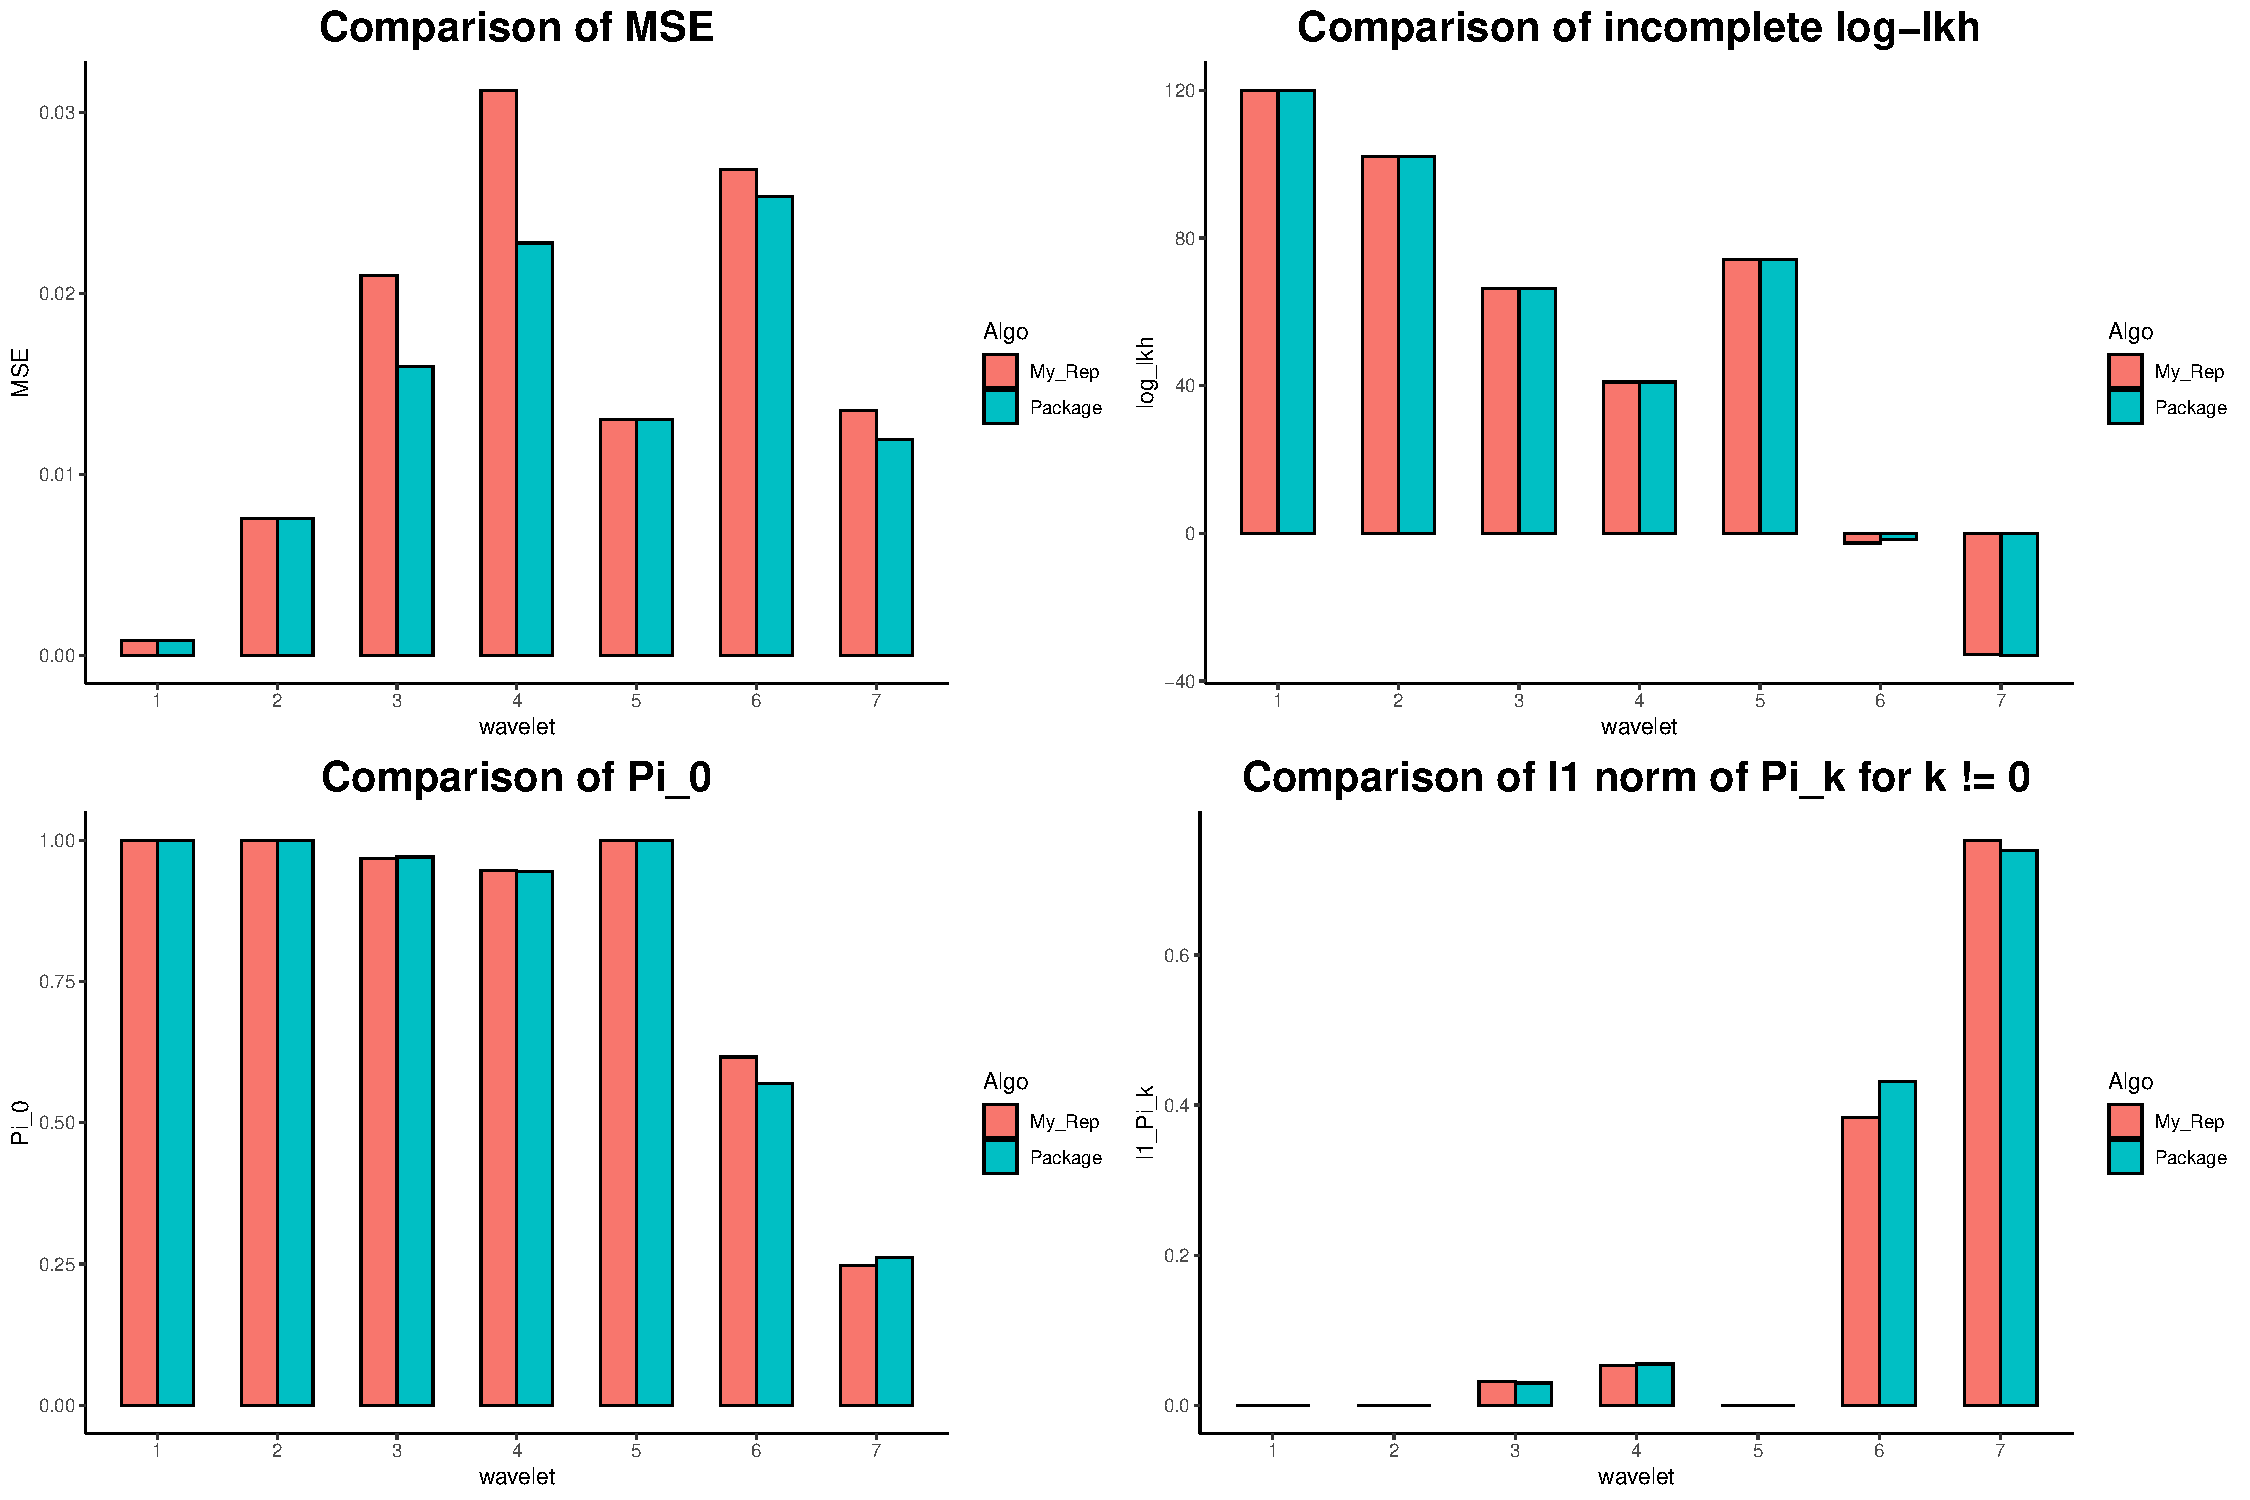
\includegraphics[width=13cm]{./plot/compare_ash.pdf}
\centering
\caption{Comparison of ASH Replication with \texttt{ash} function in Package}
\label{compare_ash}
\end{figure}

Next, comes to the results of my own replication of the \verb|SMASH| method \cite{Xing}. The procudure of data generation and "non-decimated" Wavelet Transform are the same with previous result. I compare the results of following 3 algorithms:
\begin{enumerate}[a)]
\item Applying \autoref{smash_algo} using my own replication of \verb|ASH| method.
\item Applying \autoref{smash_algo} using \verb|ash| function in \href{https://cran.r-project.org/web/packages/ashr/ashr.pdf}{\texttt{ashr}} package.
\item Directly using \verb|smash| function in \href{https://github.com/stephenslab/smashr}{\texttt{smashr}} package.
\end{enumerate} 

The MSE of the estimated posterior mean compared to the true mean of these algorithms are reported, and the resuls are shown in \autoref{compare_smash}, and the discussions of this result are provided in the subsequent subsection.

\begin{figure}[!htb]
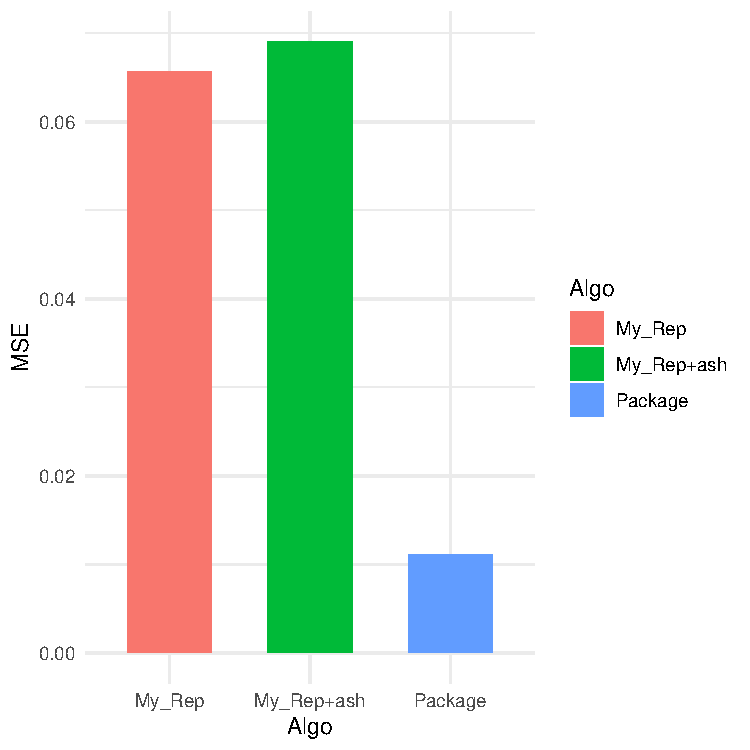
\includegraphics[width=6cm]{./plot/compare_smash.pdf}
\centering
\caption{Comparison of SMASH Replication with its Alternatives}
\label{compare_smash}
\end{figure}

\subsection{Discussion}
The \autoref{compare_ash} presents a comparison for my replication of \verb|ASH| method with the \verb|ash| function based on one realization of simulated dataset with $2^7$ data points. I also conducted checks on other realizations by setting different seeds. Notably, when $\pi_0$ is very close to $1$, the outcomes of my replication are exactly the same as those produced by the \verb|ash| function. However, when $\pi_0$ deviates from $1$, the MSE of my replication tends to be larger than that of the standard package. Nevertheless, the other quantities remain highly similar, indicating that my replication of \verb|ash| is nearly correct.

The issue with my replication for this part lies in the slow convergence of the standard EM algorithm. It is important to note that the \verb|ash| function in the \href{https://cran.r-project.org/web/packages/ashr/ashr.pdf}{\texttt{ashr}} package utilizes an accelerated EM algorithm from the \verb|R| package \href{https://cran.r-project.org/web/packages/SQUAREM/index.html}{\texttt{SQUAREM}}. Moreover, the advanced EM algorithm has the potential to achieve more accurate estimation.

The \autoref{compare_smash} presents a comparison of my replication of the \verb|SMASH| method with other alternatives mentioned in the previous subsection, based on the same simulation dataset as before. However, I encountered difficulties in replicating the \verb|SMASH| method, which could be attributed to several reasons:
\begin{enumerate}[a)]
\item The Inverse Wavelet Transform given by \eqref{inv_DWT} may not be numerically stable. Specifically, I found that the matrix $\mathbf{W}\mathbf{W}^T$ or $\mathbf{W}^{-1}\mathbf{W}$ deviates significantly from the identity matrix, with off-diagonal terms that are considerably larger than zero.
\item In my numerical experiment, the distribution approximation \eqref{SMASH_assumption5} proposed by the original paper can result in estimated variances $\hat{{\boldsymbol{s}}}^2$ being negative. This is because the domain of the Normal distribution does not necessarily exclude non-negative values. Although Appendix A of the paper provides a detailed procedure for estimating the variance, they did not mention this issue. To address this problem, I handled negative outcomes by setting them to a very small number (e.g., $1\text{e}-4$).
\item There may be additional tasks that need to be performed. For example, in Appendix B.3 of the paper, they imported \verb|MATLAB| code developed by others into \verb|R| to perform circulant shifts of the data.
\end{enumerate} 




\section{Conclusion}
This paper presents an intuitive and effective method within the Empirical Bayes framework to address the issue of homoskedasticity when estimating spatially structured mean and variance. 

The Discrete Wavelet Transform establishes a connection between the cases of sparsity and spatial structure through the property: "if the population mean of observed signals exhibits spatial structure, then its corresponding Wavelet coefficients will be sparse."

Consequently, the estimation of spatially structured mean reduces to applying Empirical Bayes techniques for sparse mean estimation on Wavelet coefficients. Similarly, the estimation of spatially structured variance involves applying Empirical Bayes techniques for sparse mean estimation on Wavelet coefficients of square of demeaned observations, while making certain distributional approximations.


\bibliography{reference}
\bibliographystyle{IEEEtran}


\end{document}